%\documentclass[tikz, border=5pt]{standalone}
\usetikzlibrary{angles, quotes, shapes.geometric} % 加载角度、引用、直角标记库
\begin{document}
	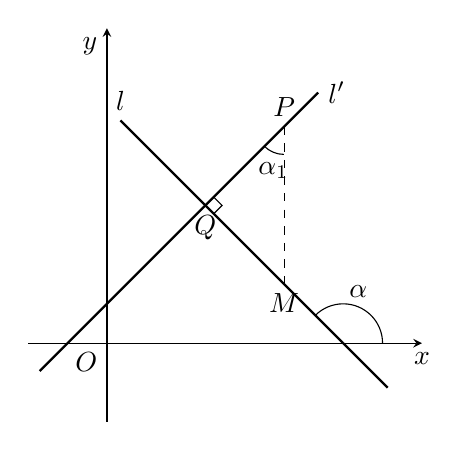
\begin{tikzpicture}[>=stealth, scale=1]
		
		% 1. 绘制坐标轴
		\draw[->] (-1,0) -- (4,0) node[below] {$x$}; % x轴(带箭头和标签)
		\draw[->] (0,-1) -- (0,4) node[below left] {$y$}; % y轴(带箭头和标签)
		\node at (0,0) [below left] {$O$}; % 原点标记
		
		% 2. 绘制直线 \( l' \)(倾斜向上)
		\draw[thick] (-0.5, 0) --  ++(45: 4.5) node[right] {$l'$};
		\draw[thick] (-0.5, 0) --  ++(-135: 0.5) ;
		
		% 3. 绘制直线 \( l \)(倾斜向下,与 \( l \) 垂直)
		\draw[thick] (3, 0) -- ++(135: 4) node[above] {$l$};
		\draw[thick] (3, 0) -- ++(-45: 0.8) ;
		
		% 4. 标记角度 \( \alpha \)(\( l \) 与 x 轴正方向的锐角)
		\draw (3.5, 0) arc (0:135:0.5)  node[midway, above] {$\alpha$};
		
		% 5. 标记角度 \( \alpha_1\)(\( l' \) 与 x 轴正方向的钝角)
		\draw (2, 2.5) arc (-135:-90:0.35) node[midway, below] {$\alpha_1$}; 
		
		% 6. 绘制直角标记(两直线垂直的符号)
		\draw (1.25, 1.75) -- ++(45: 0.15) -- ++(-45: 0.15)  -- ++(-135: 0.15) ;
		
		% 定义各关键点坐标
		\coordinate (P) at (2.25,2.75);  % 点P₁
		\coordinate (M) at (2.25, 0.75);  % 点M₁
		\coordinate (Q)  at (1.25, 1.75);% 点Q
		
		% 绘制虚线辅助线(矩形的边)
		\draw[dashed] (P) -- (M); % P₁到x轴的虚线
		
		% 标记各点的标签
		\node at (P) [above] {$P$};
		\node at (M) [below] {$M$};
		\node at (Q)  [below] {$Q$};
		
	\end{tikzpicture}
\end{document}
